%
%  =======================================================================
%  ····Y88b···d88P················888b·····d888·d8b·······················
%  ·····Y88b·d88P·················8888b···d8888·Y8P·······················
%  ······Y88o88P··················88888b·d88888···························
%  ·······Y888P··8888b···88888b···888Y88888P888·888·88888b·····d88b·······
%  ········888······"88b·888·"88b·888·Y888P·888·888·888·"88b·d88P"88b·····
%  ········888···d888888·888··888·888··Y8P··888·888·888··888·888··888·····
%  ········888··888··888·888··888·888···"···888·888·888··888·Y88b·888·····
%  ········888··"Y888888·888··888·888·······888·888·888··888··"Y88888·····
%  ·······························································888·····
%  ··························································Y8b·d88P·····
%  ···························································"Y88P"······
%  =======================================================================
% 
%  -----------------------------------------------------------------------
% Author       : 焱铭
% Date         : 2023-07-18 08:50:38 +0800
% LastEditTime : 2023-07-20 22:06:56 +0800
% Github       : https://github.com/YanMing-lxb/
% FilePath     : \GUET_Thesis_LaTeX\main.tex
% Description  : Version 0.9 更新请关注 https://github.com/GUET-TeX-Users-Group/GUET_Thesis_LaTeX
%  -----------------------------------------------------------------------
%
\special{dvipdfmx:config z 0} % XeLaTeX取消PDF压缩,加快编译速度,但会增加PDF体积
% \pdfcompresslevel=0 % PdfLaTeX取消PDF压缩,加快编译速度,但会增加PDF体积
% \pdfobjcompresslevel=0 % LuaLaTeX取消PDF压缩,加快编译速度,但会增加PDF体积
% ------------------------------------------------------------------------------------------
%     前言区域
% ------------------------------------------------------------------------------------------
\documentclass[promaster,eversion]{GUET-Thesis} 
% eversion:电子版 pversion:打印版 bachelor:本科 master:学硕 promaster:专硕 doctor:博士 ojmaster 在职硕士 ptmaster 非全专硕
% latex基础教程 lshort-zh 
% \usepackage{showframe} % 显示排版框架
% \TPshowboxestrue % 显示textblock 框架,方便调整位置
\usepackage[l2tabu, orthodox]{nag} % 检查是否有已被淘汰或过时的宏包
\graphicspath{{./Pictures/},{./Pictures/Chapter1/},{./Pictures/Chapter2/},{./Pictures/Chapter3/},{./Pictures/Chapter4/},{./Pictures/Chapter5/}} % 图片所在位置


% ------------------------------------------------------------------------------------------
%     封面信息
% ------------------------------------------------------------------------------------------
% \secrets{绝密}                                                              % 不涉密请注释该命令,不要空着
\title{基于嵌入式散热模块的微通道散热技术研究}{Research on microchannel heat dissipation technology \\& based on embedded heat dissipation module} % 题目{中文}{英文}  在标题中插入“\\&”命令进行换行
\author{焱铭}
\advisor{李XX}                                                            % 导师姓名
\protitle{教授}                                                             % 导师职称.
\school{机电工程学院}                                                        % 所在学院
\major{机械工程}                                                            % 学科专业或领域
\studentnumber{2020XXXXX}                                                   % 学号
\degreecategories{工学硕士}                                                 % 申请学位门类或类别
\datereply{\today}                                                          % 可更换为具体日期如:\datereply{2023年5月28日}


% ------------------------------------------------------------------------------------------
%     正文
% ------------------------------------------------------------------------------------------
\begin{document}
    \makecover % 封面
    % \bindpdfcover{盲审学位论文封面(示例).pdf}                              % 可使用PDF文件作为封面,如盲审封面
    \originalitydeclaration % 独创性声明
    % \signatureofdeclaration{独创性声明(示例).pdf}                          % 可使用已签字的独创性声明PDF文件
    % !Mode:: "TeX:UTF-8"


\begin{chineseabstract}
    LaTeX利用设置好的模板,可以编译为格式统一的pdf。目前国内大多出版社与高校仍在使用word,word由于其强大的功能与灵活性,在新手面对形式固定的论文时,排版、编号、参考文献等简单事务反而会带来很多困难与麻烦,对于一些需要通篇修改的问题,要想达到LaTeX的效率,对word使用者来说需要具有较高的技能水平。

    为了能把主要精力放在论文撰写上,许多国际期刊和高校都支持LaTeX的撰写与提交,新手不需要关心格式问题,只需要按部就班的使用少数符号标签,即可得到符合要求的文档。且在需要全篇格式修改时,更换或修改模板文件,即可直接重新编译为新的样式文档,这对于word新手使用word的感受来说是不可思议的。
    此项目提供用于排版桂林电子科技大学本硕博(非全,在职)毕业论文(设计)LaTeX模板类,旨在帮助桂林电子科技大学的毕业生高效地完成毕业论文的写作。

\chinesekeyword{桂林电子科技大学;本硕博学位论文;\LaTeX 模板类;\LaTeXe}
\end{chineseabstract}


\begin{englishabstract}
    LaTeX can be compiled into a pdf of uniform format using the set template.At present, most domestic publishers and universities still use word. Because of its powerful function and flexibility, when faced with fixed-form papers by novices, simple matters such as typesetting, numbering, and reference documents will bring many difficulties and troubles. For some problems that need to be modified throughout, to achieve the efficiency of LaTeX, it requires a high level of skill for word users.

    In order to focus on the writing of papers, many international journals and universities support the writing and submission of LaTeX. Novices don't need to care about formatting issues. They only need to use a few symbolic labels step by step to get the documents that meet the requirements. And when you need to modify the entire format, you can directly recompile the template file by replacing or modifying the template file. This is incredible for the word novice to use the word.


\englishkeyword{GUET; Common template; \LaTeX; \LaTeXe}
\end{englishabstract}                                              % 摘要
% ------------------------------------------------------------------------------------------   
    \thesisfigurelist                                                      % 插图目录
    \thesistablelist                                                       % 插表目录
    \thesissymbollist                                                      % 符号说明表
    \thesistableofcontents                                                 % 目录
% ------------------------------------------------------------------------------------------
    % A组表示希腊字符说明,B组为下标说明,C组为缩略词说明。
\nomenclature[C,01]{PCB}{Printed Circuit Board}
\nomenclature[C,02]{LTCC}{Low temperature cofired ceramic}
\nomenclature[C,03]{MATD}{mean absolute temperature deviation}

\nomenclature[]{$T_{f}$}{流体温度 $(K)$}
\nomenclature[]{$T_{s}$}{固体温度 $(K)$}

\nomenclature[A]{$\rho_{f}$}{流体密度 $(kg/m^3)$}
\nomenclature[A]{$\mu_{f}$}{流体动力粘度 $(kg/(m \cdot s))$}

\nomenclature[B]{$s$}{固体}
\nomenclature[B]{$f$}{流体}
% \nomenclature[B]{$$}{}                                                       % 符号定义文件

    % !Mode:: "TeX:UTF-8"
%此为第一章节。
%\figure为图片,[h]为hear代码所在,\caption为表名图名,\includegraphics为引用位置,\cite为引用参考文献,\begin{equation}公式,\subfloat子图,\label标签,\begin{table}表格,\begin{tabular}三线表,{cccc}完全居中,\toprule,\multirow取几行,\cmidrule取第几列\begin{theorem}定理,\begin{proof}证明,\begin{corollary}推论,\begin{lemma}引理
    
\chapter{绪论}\label{ch:1}
\section{节标题}

\begin{shaded}
    该部分可用于提醒自己,该段的内容中心  
    \end{shaded}

    随着人工智能和第五代移动通信技术等系统技术的发展\cite{Lau_2022},推动着半导体行业在移动便携设备、高性能计算机、自动驾驶、物联网和大数据等应用领域的发展\cite{Lau_2022},同时也推动着电子芯片向着小型化和高集成化方向发展快速发展\cite{Sadique.Murtaza.ea_2022}。
在过去的几十年里处理器上的晶体管数量依照摩尔定律\cite{Tan.Du.ea_2021}的预测呈现出指数级的增长趋势,如这张50年间的微处理器的发展趋势图(\cref{fig:processor-trend})所示。
……

\subsection{小节标题}
\subsubsection{小小节标题}

\section{图片排版示例}
\subsection{单图排版示例}

\begin{figure}[htb]
    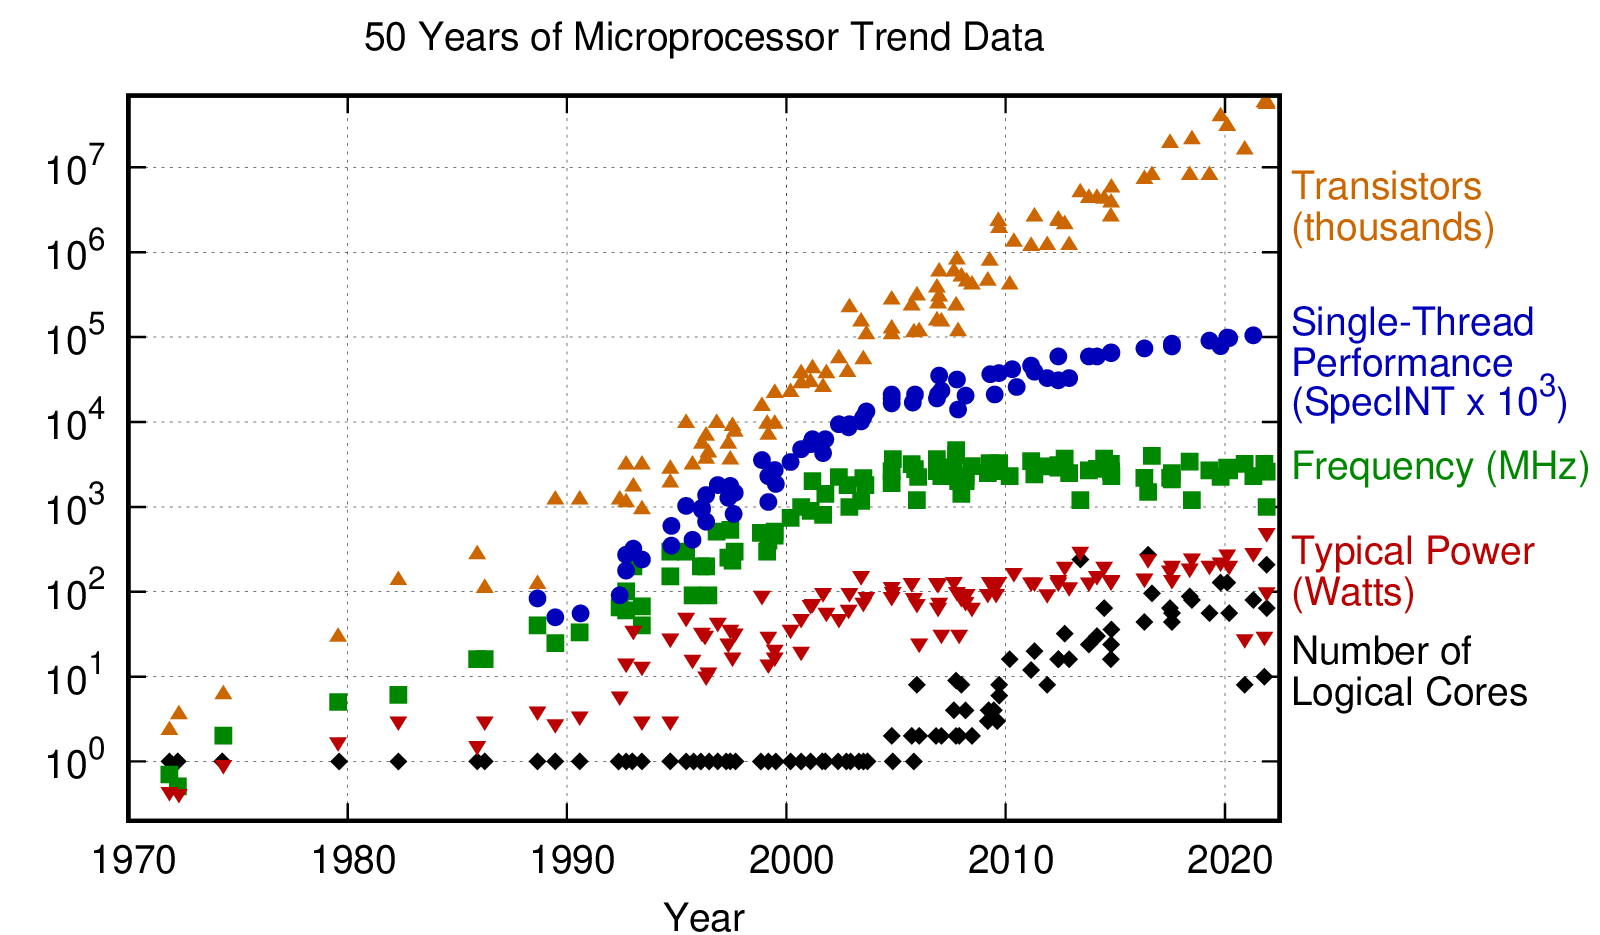
\includegraphics[width=0.8 \textwidth]{50-years-processor-trend.png}
    \caption[处理器发展]{近50年微处理器发展趋势} % 中括号中内容为插图索引中显示内容,可在题注内容过长时使用
    \label{fig:processor-trend}
\end{figure}

\subsection{多图排版示例}
同一行中的子图之间要留有空间,不要占满!否则会自动换行!

子图之间空一行表示换行。

\begin{figure}[htb]
    \subfloat[改进前的结构]{
        \label{fig:Unimproved-cooling-structure}
        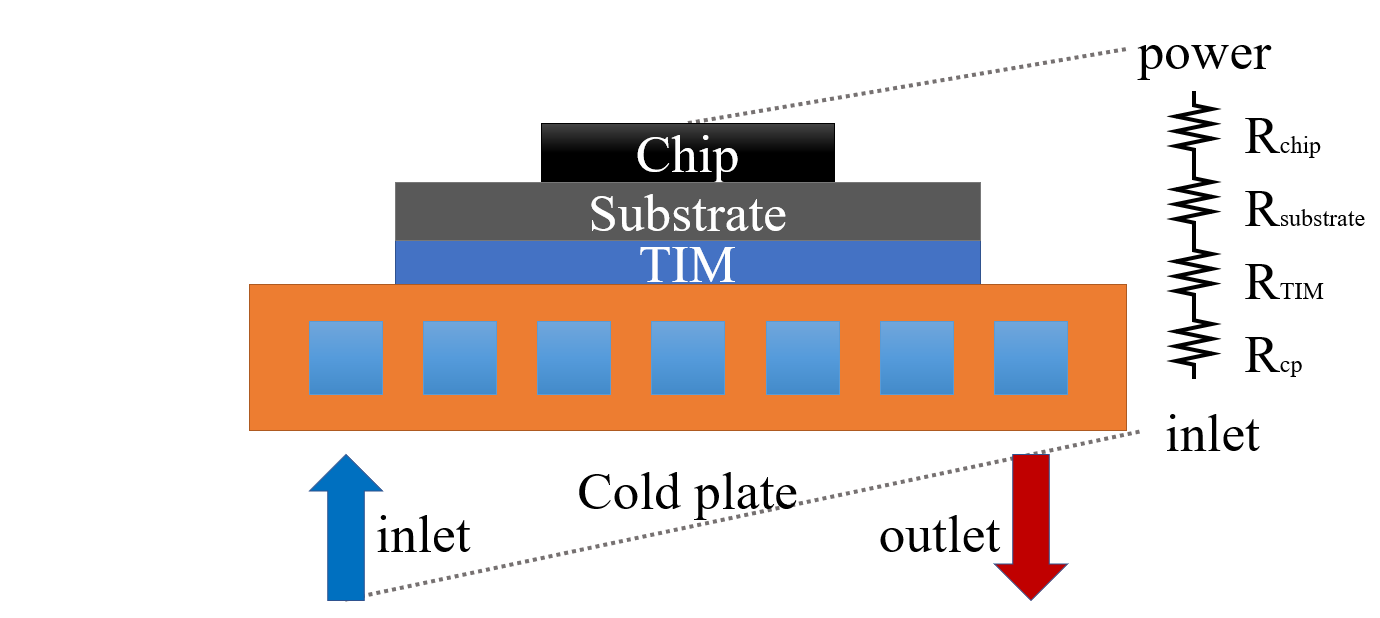
\includegraphics[width=0.45\linewidth]{Unimproved-cooling-structure.png}}
    \subfloat[基板内进行微通道散热]{
        \label{fig:LTCC-Microchannels}
        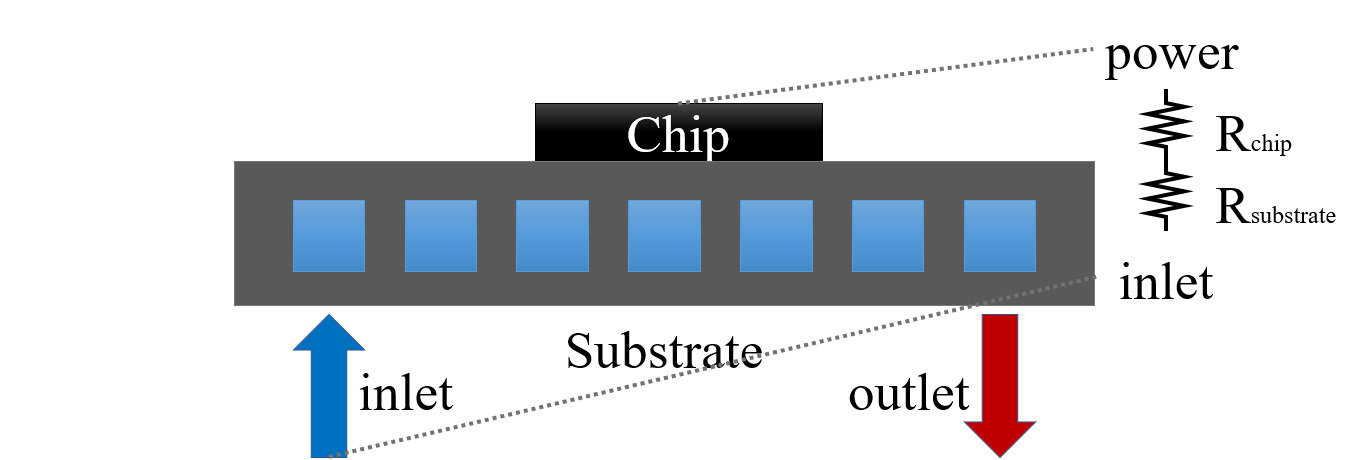
\includegraphics[width=0.45\linewidth]{LTCC-Microchannels.png}}

    \subfloat[嵌入散热模块]{
        \label{fig:Embedded-cooling-module}
        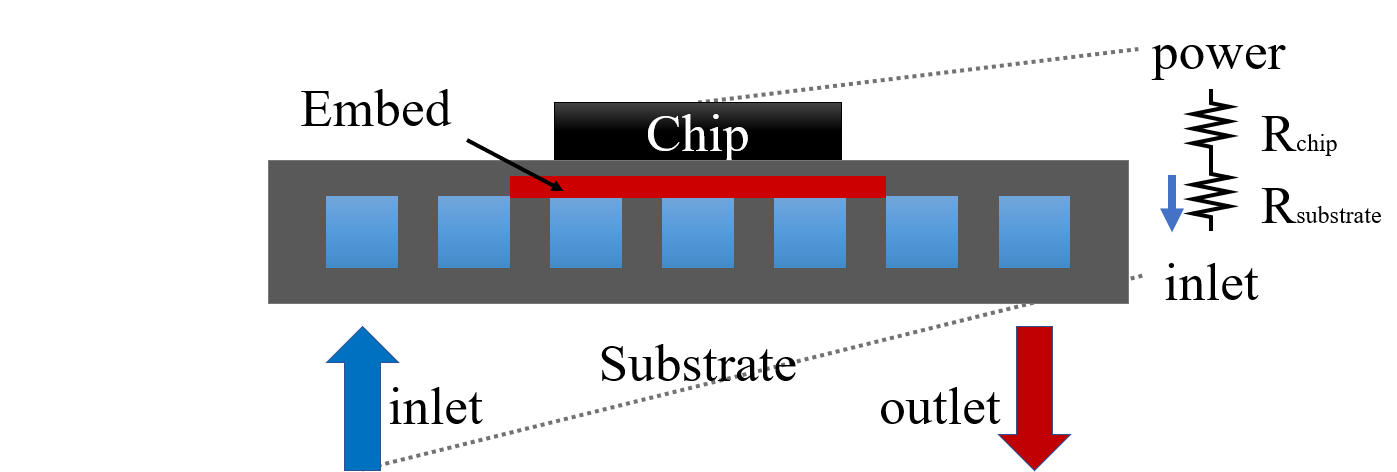
\includegraphics[width=0.45\linewidth]{Embedded-cooling-module.png}}
    \subfloat[带针鳍或肋的嵌入式散热模块]{
        \label{fig:Rib-pin-fin}
        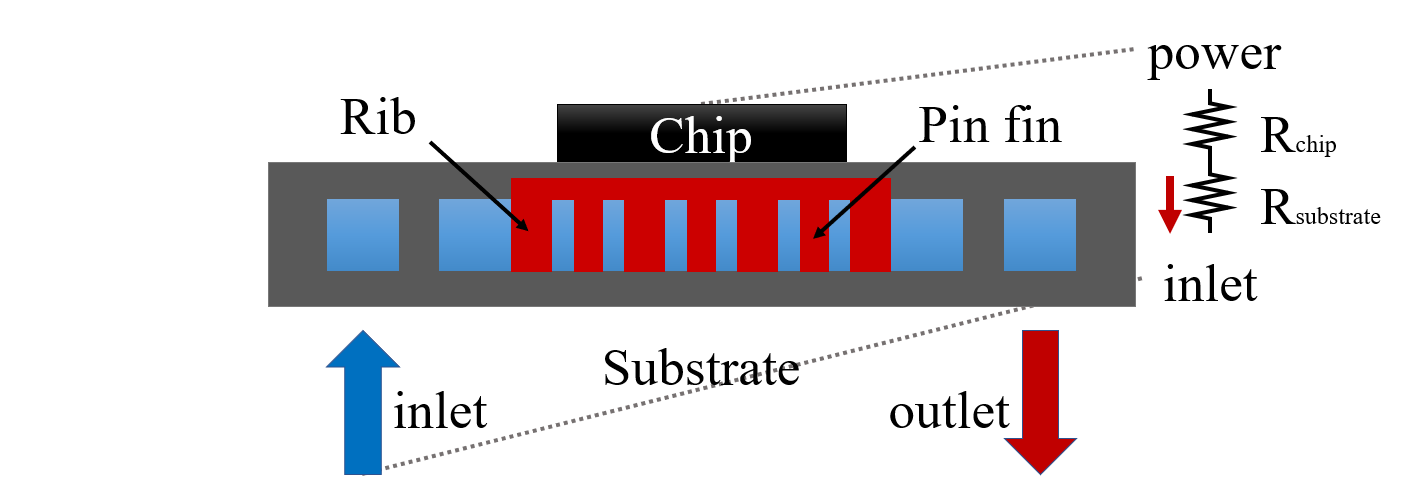
\includegraphics[width=0.45\linewidth]{Rib-pin-fin.png}}
    \caption{三种强化传热途径示意图}
    \label{fig:Three-enhanced-heat-transfer-paths}
\end{figure}


\section{本论文的结构安排}
\cref{ch:1}:绪论。本章主要分为……。

\cref{ch:2}:相关理论基础及结构设计要求与思路。本章主要分为……。

\cref{ch:3}:基于嵌入式散热模块的微通道流动与传热性能研究。本章研究了几种……。

\cref{ch:4}:基于嵌入式散热模块的微通道多目标优化分析。本章在\cref{ch:3}完成基于……。

\cref{ch:5}:基于MC-RPF的多热源散热结构设计分析及压降优化。本章在\cref{ch:4}完成MC-RPF多目标优化……。

\cref{ch:6}:全文总结与展望。本次研究工作进行总结,并根据全文研究过程中……。



    % !Mode:: "TeX:UTF-8"
%此为章节二模板
%\chapter、\section、\subsection、\subsubsection分别对应一二三四级标题
\chapter{图片示例}\label{ch:2}

\section{图片排版示例}
\textbf{注意}:使用\textbackslash caption[]\{\}命令时,如果不需要设置缩写目录的内容,一定要删掉[],否则插图插表索引将不会显示该图或表的目录。

\textbf{建议}:在论文写作时图片位置可以先按照写作时的习惯进行放置,待到完成所有写作内容后再进行详细调整图片位置。

\subsection{图片格式}

\LaTeX 中图片推荐使用pdf格式。使用Origin可导出矢量无白边的图片以保证清晰度,其次推荐使用jpg,png格式图片。

为了保证图片的清晰,jpg图片导出时ppi建议设置为300,png图片导出时建议宽度设置为1024像素(可根据需求自行设置),长度随宽度变化。

\subsection{单图排版示例}

\begin{figure}[htb]
    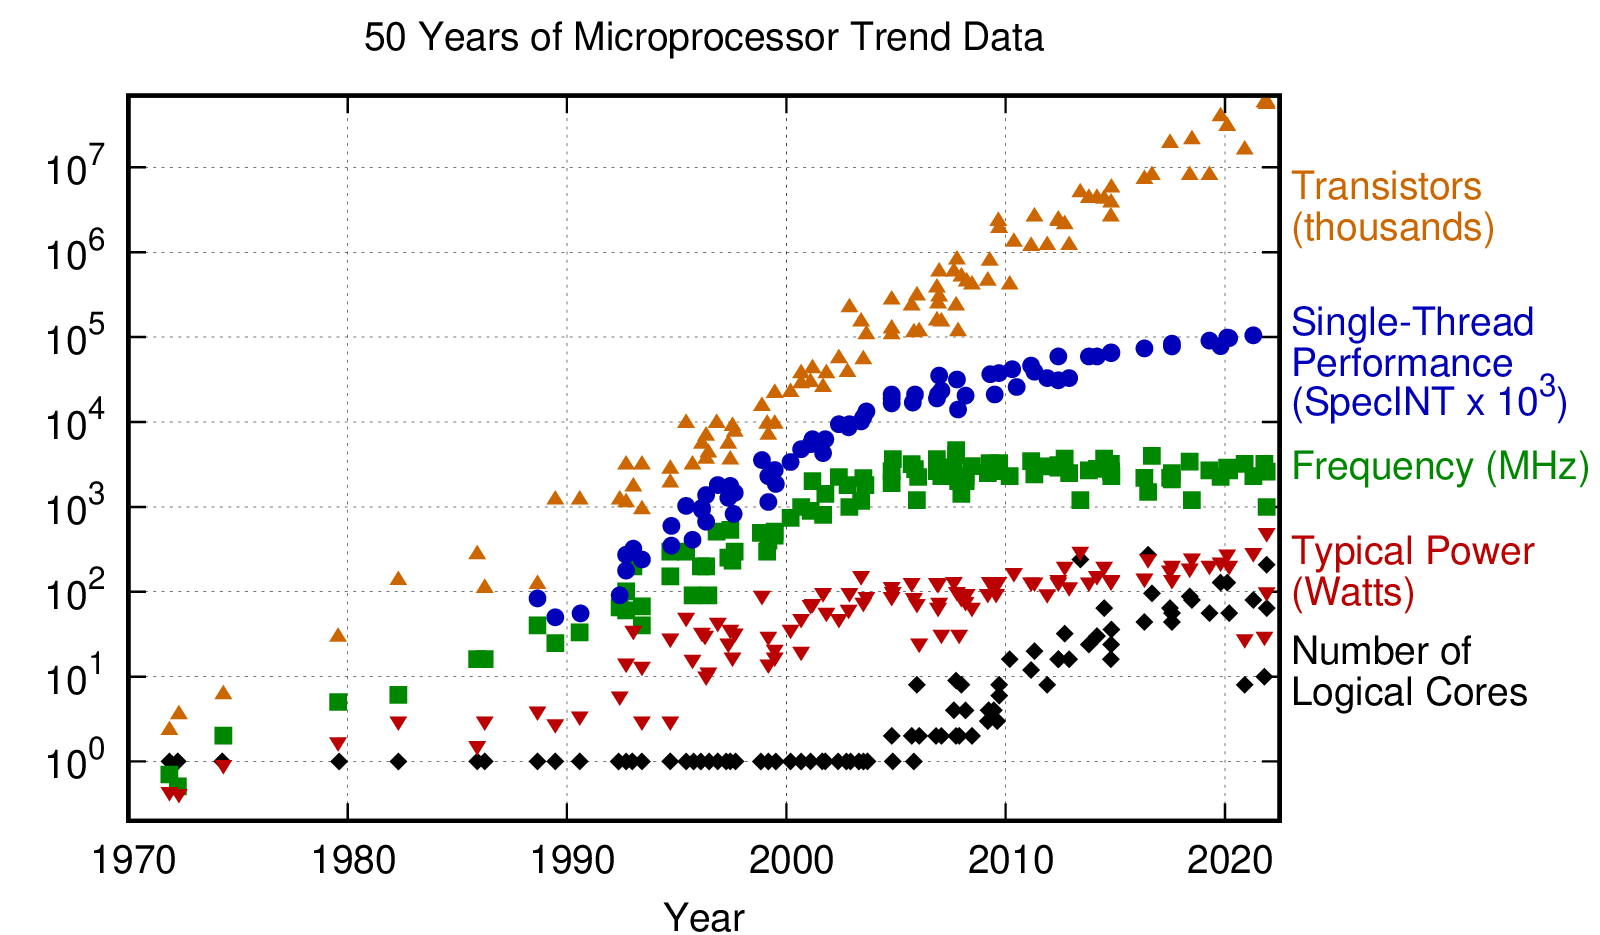
\includegraphics[width=0.8 \textwidth]{50-years-processor-trend.png}
    \caption[处理器发展]{近50年微处理器发展趋势} % 中括号中内容为插图索引中显示内容,可在题注内容过长时使用
    \label{fig:processor-trend}
\end{figure}

图片引用示例:\cref{fig:processor-trend}。

\subsection{多图排版示例}
同一行中的子图之间要留有空间,不要占满!否则会自动换行!

子图之间空一行表示换行。

插入子图请使用\textbackslash subfloat\{\}命令。

\begin{figure}[htb]
    \subfloat[改进前的结构]{
        \label{fig:Unimproved-cooling-structure}
        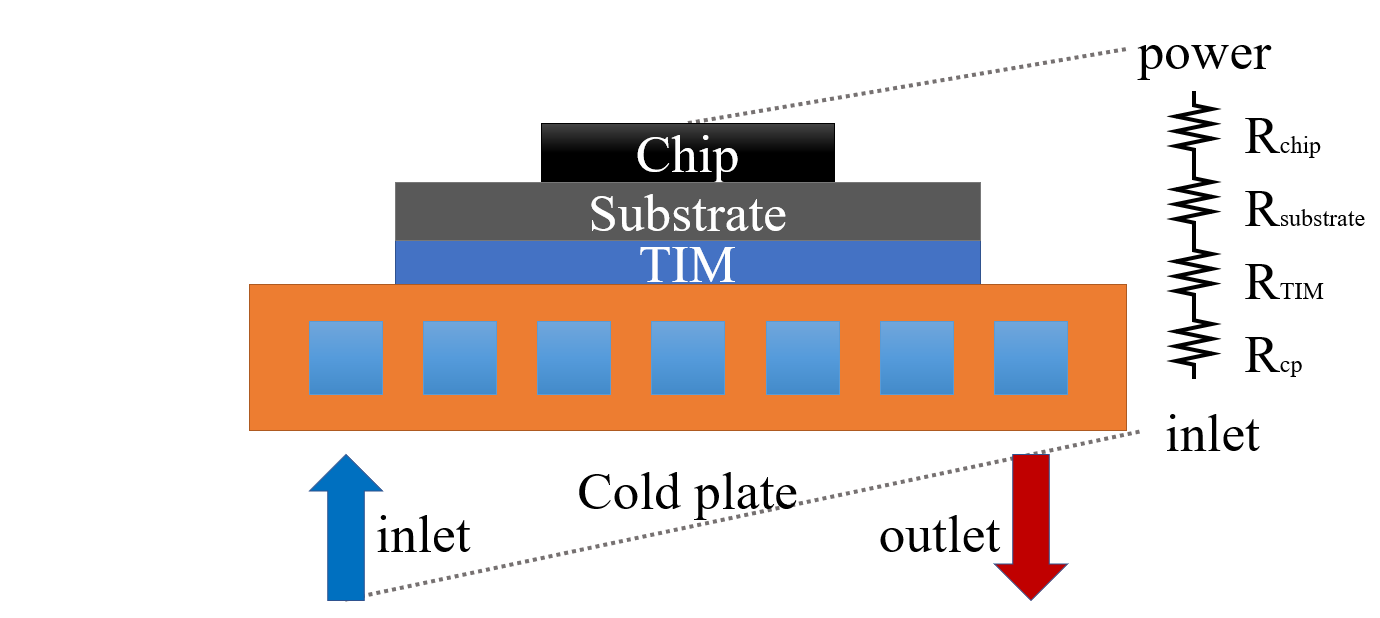
\includegraphics[width=0.45\linewidth]{Unimproved-cooling-structure.png}}
    \subfloat[基板内进行微通道散热]{
        \label{fig:LTCC-Microchannels}
        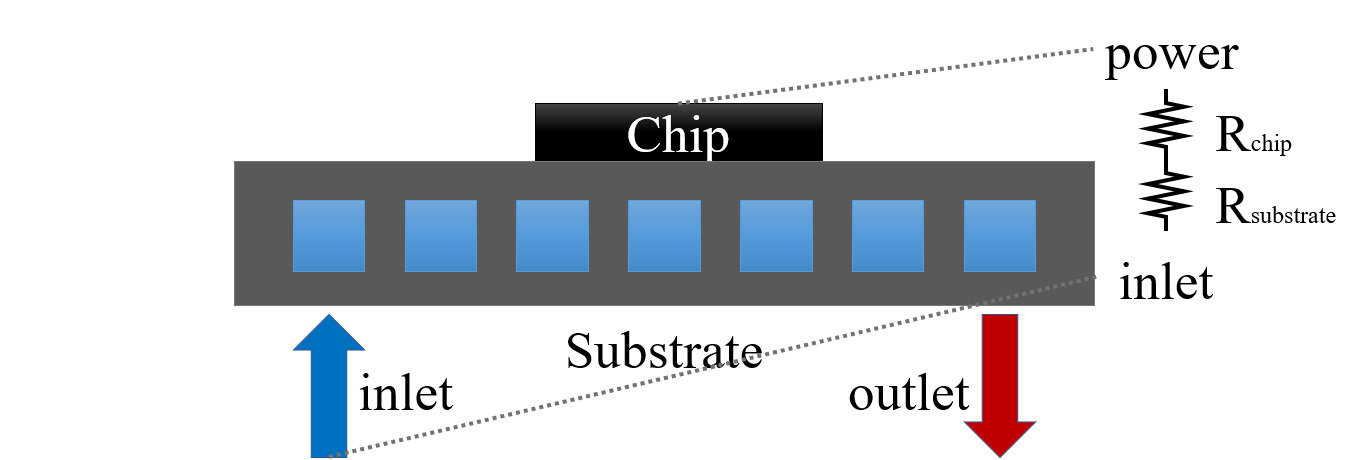
\includegraphics[width=0.45\linewidth]{LTCC-Microchannels.png}}

    \subfloat[嵌入散热模块]{
        \label{fig:Embedded-cooling-module}
        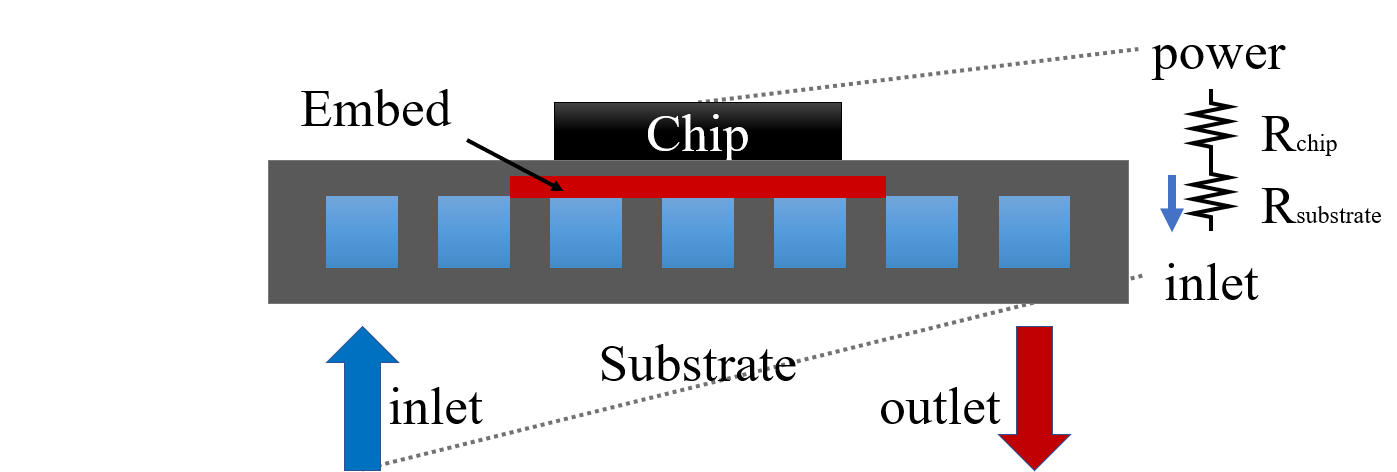
\includegraphics[width=0.45\linewidth]{Embedded-cooling-module.png}}
    \subfloat[带针鳍或肋的嵌入式散热模块]{
        \label{fig:Rib-pin-fin}
        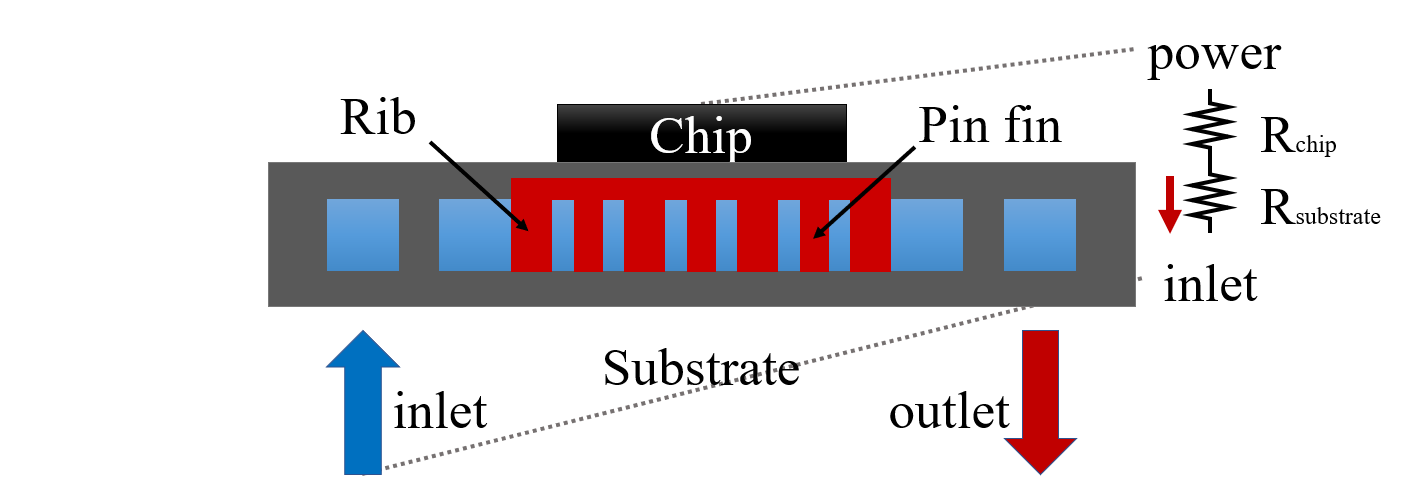
\includegraphics[width=0.45\linewidth]{Rib-pin-fin.png}}
    \caption{三种强化传热途径示意图}
    \label{fig:Three-enhanced-heat-transfer-paths}
\end{figure}

子图引用示例:\cref{fig:Unimproved-cooling-structure},

整图引用示例:\cref{fig:Three-enhanced-heat-transfer-paths}。

\section{本章小节}
本章介绍了基于嵌入式散热模块的微通道散热技术所涉及的基……
    % !Mode:: "TeX:UTF-8"

\chapter{基于嵌入式散热模块的微通道流动与传热性能研究}\label{ch:3}

\section{公式示例}
在本次研究中应用到计算流体动力学(Computational Fluid Dynamics,CFD)对研究对象进……。


\subsection{普通带序号公式}
\begin{equation}
    \frac{\partial u}{\partial x}+\frac{\partial v}{\partial y}+\frac{\partial v}{\partial z}=0
\end{equation}
u,v,w 分别是 x,y,z 方向的速度分量。


\subsection{需要对齐的多个带序号的公式}

\&号为对其对齐标记最好放置在计算符号之前,如=、+、-之前;

\textbackslash\textbackslash 表示换行。

\begin{align}% 式中的&为对齐的位置标记
    u & \frac{\partial u}{\partial x}+v \frac{\partial u}{\partial y}+w \frac{\partial u}{\partial z}=-\frac{1}{\rho_{f}} \frac{\partial p}{\partial x}+\frac{\mu_{f}}{\rho_{f}}\left(\frac{\partial^{2} u}{\partial x^{2}}+\frac{\partial^{2} u}{\partial y^{2}}+\frac{\partial^{2} u}{\partial z^{2}}\right) \\
    u & \frac{\partial v}{\partial x}+v \frac{\partial v}{\partial y}+w \frac{\partial v}{\partial z}=-\frac{1}{\rho_{f}} \frac{\partial p}{\partial y}+\frac{\mu_{f}}{\rho_{f}}\left(\frac{\partial^{2} v}{\partial x^{2}}+\frac{\partial^{2} v}{\partial y^{3}}+\frac{\partial^{2} v}{\partial z^{3}}\right) \\
    u & \frac{\partial w}{\partial x}+v \frac{\partial w}{\partial y}+w \frac{\partial w}{\partial z}=-\frac{1}{\rho_{f}} \frac{\partial p}{\partial z}+\frac{\mu_{f}}{\rho_{f}}\left(\frac{\partial^{2} w}{\partial x^{2}}+\frac{\partial^{2} w}{\partial y^{2}}+\frac{\partial^{2} w}{\partial z^{2}}\right)
\end{align}
$\rho_{f}$ 和 $\mu_{f}$ 分别是冷却剂的密度和动态粘度,p 是冷却剂压力。


\subsection{需要换行对齐的长公式}

\begin{equation}\label{eq:P}
    \begin{split}
        f_3 & = 6.272 + 3.02 H_{rib} + 6.08 H_{pf} + 0.0368 N_{pf} - 0.8848 N_{ac} + 0.04381 N_{ac}^2\\
        & + 6.35 H_{rib} \times H_{pf} - 0.3602 H_{rib}\times N_{ac} - 0.5497 H_{pf}\times N_{ac}
    \end{split}
\end{equation}

\subsection{其他公式示例}
\begin{equation}
    \begin{aligned}
    \left\{
        \begin{array}{l}
        \text {find}\enspace H_{rib},H_{rib},N_{pf},N_{ac} \\
        \text {min} \enspace F(H_{rib},H_{rib},N_{pf},N_{ac})= min\{f_1,f_2,f_3\} \\

            \text{s.t.\enspace}\enspace 0.2 \leqslant H_{rib} \leqslant 0.8    \\
            \hspace{2.2em} 0.2 \leqslant H_{pf} \leqslant 0.8                     \\
            \hspace{2.2em} 6 \leqslant N_{pf} \leqslant 22,\ N_{pf}\in \mathbb{O} \\
            \hspace{2.2em} 0 \leqslant N_{ac} \leqslant 16,\ N_{ac}\in \mathbb{E}
        \end{array}
    \right. 
    \end{aligned}
    \label{eq:MO}
\end{equation}
    % !Mode:: "TeX:UTF-8"

\chapter{基于嵌入式散热模块的微通道多目标结构优化}\label{ch:4}

\section{概述}
本章在\cref{ch:3}完成基……。

\section{列表示例}\label{sec:enumerate}

\subsection{普通列表示例}
\begin{enumerate}
    \item 在基板内部进行微通道散热以缩短传热路径,见\cref{fig:LTCC-Microchannels};
    \item 在基板内嵌入散热模块减少整体热阻,提高热传导效率,见\cref{fig:Embedded-cooling-module};
    \item 在嵌入式散热模块上制作针鳍或肋增强对流传热,以进一步减小热阻,见\cref{fig:Rib-pin-fin}。
\end{enumerate}

\subsection{标号为阿拉伯数字的列表}

\begin{enumerate}[label =(\arabic*)]

    \item 基于嵌入式散热模块的微通道流动与传热性能研究。
          将三种带有嵌入式散热模块的微通道:带有针鳍……
          最终选用MC-RPF作为核心散热结构;
    \item 分析几何参数对带有针鳍-肋嵌入式散热模块微通道流动与传热的影响。
          主要研究……;
    \item 对采用针鳍-肋嵌入式散热模块的微通道进行多目标优化。
          采用响应面分析法(Response Surface Methodology,RSM)与……;
    \item 基于MC-RPF的多热源散热结构设计分析。
          为解决在多热源应……;
    \item 基于MC-RPF的多热源散热结构压降优化。
          以压降损失相关理论为指导依据,……。

\end{enumerate}

\subsection{自定义列表标号}
\noindent NSGA-Ⅱ具体操作步骤如下:
\begin{enumerate}[leftmargin = 6em, labelsep = 0em]
    \item[步骤一、] 随机生成初始化种群,设置代数$Gen = 0$;
    \item[步骤二、] 判断是否生成第一代种群,如已生成则令其代数$Gen = 2$,否则进行快速非支配排序、选择、SBX、PM生成第一代子群,并设置代数$Gen = 2$;
    \item[步骤三、] 将父代与子代的种群进行合并形成新的父代种群;
    \item[步骤四、] 判断是否生成新的父代种群,如果未生成则进行快速非支配排序、拥挤度计算、精英策略选择操作以生成新的父代;
    \item[步骤五、] 对新生成的父代进行选择、SBX、PM操作生成新子群;
    \item[步骤六、] 判断当前代数是否小于设置的最大代数,若小于设置的最大代数则返回步骤三进行循环,否则,NSGA-Ⅱ结束运行。
\end{enumerate}

\section{本章小节}
    %
%  =======================================================================
%  ····Y88b···d88P················888b·····d888·d8b·······················
%  ·····Y88b·d88P·················8888b···d8888·Y8P·······················
%  ······Y88o88P··················88888b·d88888···························
%  ·······Y888P··8888b···88888b···888Y88888P888·888·88888b·····d88b·······
%  ········888······"88b·888·"88b·888·Y888P·888·888·888·"88b·d88P"88b·····
%  ········888···d888888·888··888·888··Y8P··888·888·888··888·888··888·····
%  ········888··888··888·888··888·888···"···888·888·888··888·Y88b·888·····
%  ········888··"Y888888·888··888·888·······888·888·888··888··"Y88888·····
%  ·······························································888·····
%  ··························································Y8b·d88P·····
%  ···························································"Y88P"······
%  =======================================================================
% 
%  -----------------------------------------------------------------------
% Author       : 焱铭
% Date         : 2023-12-03 15:43:39 +0800
% LastEditTime : 2025-01-14 20:54:49 +0800
% Github       : https://github.com/YanMing-lxb/
% FilePath     : /GUET_Thesis_LaTeX/Chapters/Chapter5.tex
% Description  : 
%  -----------------------------------------------------------------------
%

% !Mode:: "TeX:UTF-8"

\chapter{算法与定理的示例}\label{ch:5}

\section{算法示例}

\noindent 算法示例如下:

% \begin{algorithm}[H]
%     \KwData{this text}
%     \KwResult{how to write algorithm with \LaTeX2e}
%     initialization\;
%     \While{not at end of this document}{
%         read current\;
%         \eIf{understand}{
%             go to next section\;
%             current section becomes this one\;
%         }{
%             go back to the beginning of current section\;
%         }
%     }
%     \caption{How to wirte an algorithm.}
%     \label{alg:my_algorithm}
% \end{algorithm}

% 算法如\cref{alg:my_algorithm}

\begin{figure}
    \begin{mdframed}
    \begin{multicols}{2}
        \begin{algorithmic}[1] %每行显示行号
            \scriptsize
            \While{由 CS 使用输入 $1^\lambda$ 进行调用}
                \While{从 CS 接收 $1^\lambda$} \textcolor{blue}{\Comment{$\mathsf{Init}$}}
                    \State \textbf{return} $pp = (\mathbb{G}, \mathbb{Z}^{*}_{p}, p, \mathsf{g}, H, \mathcal{H}, \mathsf{PRG})$
                \EndWhile
                \Statex
                
                \While{从 CS 接收 $pp$} \textcolor{blue}{\Comment{$\mathsf{KeyGen_{par}}$}}
                    \For{$i \gets 1 \ \mathbf{to} \ n$} \Comment{$u_i$}
                        \State $(\mathtt{X}_{i}, \mathtt{x}_{i}) \leftarrow \mathcal{MKEM}.\mathsf{Gen}(pp)$
                        \State $a_i \overset{\$}{\leftarrow} \mathbb{Z}^{*}_{p}, y_i \leftarrow \mathsf{g}^{a_i}$
                        \State $pk_i \leftarrow (y_i, \mathtt{X}_{i}), sk_i \leftarrow (a_i, \mathtt{x}_{i})$
                        \State \textbf{Send} $( u_i, \mathtt{X}_{i} )$ to CS
                    \EndFor
                    \If{$|u_i| = n$}  \Comment{CS}
                        \State $\{u_i \in U\}$.sort()
                        \State $u_i \leftarrow \{ u_i, \mathtt{X}_{i} \}_{u_i \in U}$
                    \EndIf
                \EndWhile
                \Statex
                
                \While{从 CS 接收 $pp$} \textcolor{blue}{\Comment{$\mathsf{KeyGen_{cs}}$}}
                    \State $(\mathtt{pk}, \mathtt{sk}) \leftarrow \mathcal{MKEM}.\mathsf{Gen}(pp)$ \Comment{CS}
                    \State $\nu \overset{\$}{\leftarrow} \mathbb{Z}^{*}_{p},  \mu \leftarrow \mathsf{g}^{\nu}$
                    \State $pk \leftarrow (\mathtt{pk}, \mu), sk = (\mathtt{sk}, \nu)$
                \EndWhile
                \Statex
                
                \While{从 $u_{i}$, CS 接收 $(\{pk_{i} | i \in n\}, pk)$} \textcolor{blue}{\Comment{$\mathsf{SekeyGen}$}}
                    \For{$i \gets 1 \ \mathbf{to} \ n$} \Comment{$u_i$}
                        \For{$j \gets 1 \ \mathbf{to} \ n, j \neq i$}
                            \State $(KU_{i,j}, CU_{i,j}) \leftarrow \mathcal{MKEM}.\mathsf{Enc}(\mathcal{Q}_{i,j})$
                            \State \textbf{Send} $\{(CU_{i,j}, u_i, u_j) | u_{i}, u_{j} \in U , i \neq j\}$
                        \EndFor
                    \EndFor
                    \For{$i \gets 1 \ \mathbf{to} \ n$} \Comment{CS}
                        \For{$j \gets i + 1 \ \mathbf{to} \ n$}
                            \State $(K_{i,j}, C_{i,j}) \leftarrow \mathcal{MKEM}.\mathsf{Enc}(\mathcal{P}_{i,j})$
                            \State \textbf{Send} $\{(C_{i,j}, u_i, u_j) | u_{i}, u_{j} \in U , i \neq j\}$
                        \EndFor
                    \EndFor
                \EndWhile
                \Statex
                
                \While{从 $u_{i}$, CS 接收 $(sk_{i}, sk, pk_{i}, pk)$} \textcolor{blue}{\Comment{$\mathsf{ThrNegKey}$}}
                    \For{$i \gets 1 \ \mathbf{to} \ n$} \Comment{$u_i$}
                        \For{$j \gets 1 \ \mathbf{to} \ n, j \neq i$}
                            \State $KU_{j,i} \leftarrow \mathcal{MKEM}.\mathsf{Dec}(CU_{j,i}, \mathtt{x}_{i}, \mathcal{Q}_{j,i})$
                            \State $K_{i,j} \leftarrow \mathcal{MKEM}.\mathsf{Dec}(C_{i,j}, \mathtt{x}_{i}, \mathcal{P}_{i,j})$
                        \EndFor
                    \EndFor
                    \For{$i \gets 1 \ \mathbf{to} \ n$} \Comment{CS}
                        \For{$j \gets i + 1 \ \mathbf{to} \ n$}
                            \State $KU_{i,j} \leftarrow \mathcal{MKEM}.\mathsf{Dec}(CU_{i,j}, \mathtt{sk}, \mathcal{Q}_{i,j})$
                            \State $KU_{j,i} \leftarrow \mathcal{MKEM}.\mathsf{Dec}(CU_{j,i}, \mathtt{sk}, \mathcal{Q}_{j,i})$
                        \EndFor
                    \EndFor
                    \State $\mathbf{k}_{i,j} \leftarrow \mathsf{PRG}(KU_{j,i} \| sid) \oplus \mathsf{PRG}(KU_{i,j} \| sid) \oplus \mathsf{PRG}(K_{i,j} \| sid)$ \Comment{$u_{i}$, CS}
                \EndWhile
                \Statex
                
                \While{从 $u_{i}$ 接收 $\mathbf{k}_{i,j}, m_i$} \textcolor{blue}{\Comment{$\mathsf{MaskIn}$}}
                    \For{$i \gets 1 \ \mathbf{to} \ n$} \Comment{$u_i$}
                        \For{$j \gets 1 \ \mathbf{to} \ n, j \neq i$}
                            \State $\hat{m}_i \leftarrow m_i + \sum_{u_i < u_j} \mathsf{PRG}(\mathbf{k}_{i,j}) - \sum_{u_i > u_j} \mathsf{PRG}(\mathbf{k}_{i,j})$
                        \EndFor
                    \EndFor
                \EndWhile
                \Statex

                \State 后文省略...

            \EndWhile
%				\EndFunction
        \end{algorithmic}
    \end{multicols}
    \end{mdframed}
    \caption[方案一伪代码]{方案的伪代码}
    \label{fig_algo}
\end{figure}

该方案的过程在\cref{fig_algo}中描述。这种算法常用于写方案的总览

第二种算法示例如下:

\begin{algorithm}[!htbp]
    \caption{承诺批量验证与错误检测}
    \label{algo_find_err}
    \begin{algorithmic}[1] %每行显示行号
        \Require $\mathsf{Com}^{\mathsf{Agg}}_{j}$,其中 $i \in [1,n]$
        \Ensure  $(\mathsf{flag}, l)$
        \Function {ComBatchVali and ErrDete}{$\mathsf{Com}^{\mathsf{Agg}}_{j},\{\mathsf{g}^{[\![ \hat{x}_{i} ]\!]_{j}}h^{[\![ \ell_{i} ]\!]_{j}}\}_{i \in [1,n]}$}
        \For{$i \gets 1 \ \mathbf{to} \ n$}
            \State $T_1[i + n - 1] = \mathsf{Com}^{\mathsf{Agg}}_{j}$
            \State $T_2[i + n - 1] = \mathsf{g}^{[\![ \hat{x}_{i} ]\!]_{j}}h^{[\![ \ell_{i} ]\!]_{j}}$
        \EndFor
        \While{!$q$.empty()}
            \If{$a < n$}
                \State $q$.push($2a$), $q$.push($2a + 1$)
            \Else
                \State $l$.add($a - n + 1$)
            \EndIf
        \EndWhile
        \EndFunction
    \end{algorithmic}
\end{algorithm}

算法的引用也是\cref{algo_find_err}的形式。

\section{定理定义示例}

\begin{theorem}
    XXXXXXXXXX
\end{theorem}
\begin{proof}
    XXXXXXXXXX
\end{proof}
\begin{corollary}
    XXXXXXXXXX
\end{corollary}
\begin{lemma}
    XXXXXXXXXX
\end{lemma}

提供了大量额外的定理环境,如定义、注释、例子等,可以根据需要自行添加。
\begin{verbatim}
    \begin{theorem} % 定理
        XXXXXXXXXX
    \end{theorem}
    \begin{axiom} % 公理
        XXXXXXXXXX
    \end{axiom}
    \begin{corollary} % 推论
        XXXXXXXXXX
    \end{corollary}
    \begin{lemma} % 引理
        XXXXXXXXXX
    \end{lemma}
    \begin{definition} % 定义
        XXXXXXXXXX
    \end{definition}
    \begin{example} % 例子
        XXXXXXXXXX
    \end{example}
    \begin{proposition} % 命题
        XXXXXXXXXX
    \end{proposition}
    \begin{assertion} % 断言
        XXXXXXXXXX
    \end{assertion}
    \begin{assumption} % 假设
        XXXXXXXXXX
    \end{assumption}
    \begin{agreement} % 协议
        XXXXXXXXXX
    \end{agreement}
\end{verbatim}

且均支持自动编号和引用,如 \verb|\cref{thm:1}、\cref{cor:1}、\cref{lem:1}|、\verb|\cref{def:1}、\cref{exm:1}|


                                              % 可根据需求自行添加章节数

    % !Mode:: "TeX:UTF-8"

\chapter{全文总结与展望}\label{ch:6}

\section{全文总结}
\section{空白符号}
    % 空行分段,多个空行等同于一个
    % 自动缩进,绝对不能使用空行代替
    % 英文中多个空格处理为一个空格,中文中空格会被忽略
    % 汉字与其他字符的间距会自动有XeLaTeX处理
    % 禁止使用中文全角空格
 
    % 1em(当前字体中M的宽度)
    1em: a\quad b
 
    % 2em
    2em: a\qquad b
 
    % 约为1/6个em
    1/6个em: a\,b 或 a\thinspace b
 
    % 0.5个em
    0.5个em: a\enspace b
 
    % 空格
    空格: a\ b
 
    % 硬空格,即不能分割的空格
    硬空格: a~b
 
    % 1pc=12pt=4.218mm
    指定宽度1pc: a\kern 1pc b
 
    指定宽度-1em: a\kern -1em b
 
    指定宽度1em: a\hskip 1em b
 
    指定宽度35pt: a\hspace{35pt}b
 
    % 占位宽度
    占位宽度为xyz: a\hphantom{xyz}b
 
    % 弹性长度hfill命令用于撑满整个空间
    弹性长度: a\hfill b

\section{\LaTeX 控制符}
\#              % 输出井号
\$              % 输出美元符号
\{ \}           % 输出大括号
\~{}            % 输出波浪
\_{}            % 输出下划线
\^{}            % 输出尖角
\textbackslash  % 输出反斜杠
\&              % 输出与符号


\section{后续工作展望}                                            % 总结与展望
% ------------------------------------------------------------------------------------------
    \thesisbibliography{./References/reference.bib}                        % 参考文献
    % 默认调用GUET-Thesis(base-gbt7714-numerical)参考文献样式,当参考文献数目超过100时,可以使用large选项调整编号
    % 如\thesisbibliography{large}{./References/reference.bib} 

% ------------------------------------------------------------------------------------------
    % 此处一般不用,除非要自定义参考文献样式,更换参考文献样式文件
    % \bibliographystyle{GUET-Thesis(base-gbt7714-numerical)}              % 自定义参考文献样式
    % \bibliography{reference} % 参考文献库
% ------------------------------------------------------------------------------------------
    \thesisacknowledgement                                                 % 致谢
    \thesisaccomplish                                                      % 攻读专业硕士学位期间取得的成果
    
\end{document} 
